\chapter{Application design and implementation}\label{sec:ApplicationDesingAndImplementation}
This chapter describes all important information about created application. First is hardware and software used for developing and testing of the application. Second is structure and description of core parts used in the application. 

\begin{figure}[H]
	\begin{centering}
		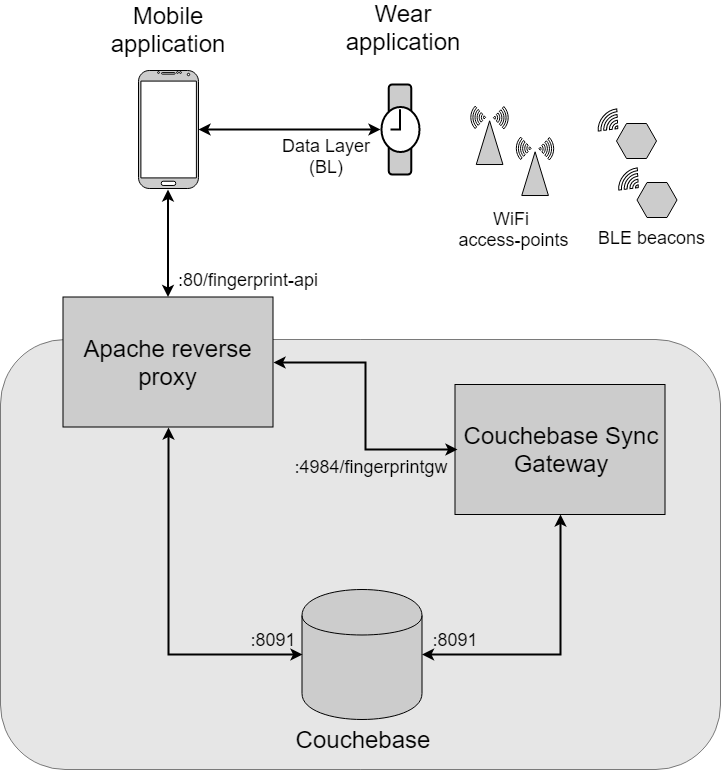
\includegraphics[width=0.6\textwidth]{img/server_architecture}
		\par\end{centering}
	\caption{Application architecture (based on \cite{IILUBLEB})}
	\label{fig057}
\end{figure}

\fref{fig057} shows basic devices and technologies used in this application. There are three main part of this implementation, mobile, wear and server application. Mobile and wear parts implement scanning for radio signals and are written in Java language for Android system. Server is also programmed in Java to keep implementations close to each other and make future adjustments easier. Main goal of the server is to store scanned data.

\section{Hardware}\label{sec:Hardware}
There are multiple hardware devices used in this application. All of them can be seen on \fref{fig057}, where first and the most obvious are smartphone and smartwatch. These devices scan radio signals from WiFi access-points and BLE beacons that are placed in the indoor environment. And a final hardware part is a server holding scanned data from all devices.

\subsection{Smartphone and Smartwatch}\label{subsec:SmartphoneAndSmartWatch}
Both smart devices must support scanning of Bluetooth Low Energy beacons that can be done with Bluetooth 4.0 and higher. Secondary requirements are Wi-Fi, GSM and LTE modules to support more data types than just BLE beacons.

\subsubsection{Phone}\label{subsubsec:Phone}
Main part of the application is developed and tested on Redmi Note 4 from Chinese company Xiaomi. It is running customized version of Android 6.0 called MIUI. Even thought system was customized, in core it is still Android so there are no problems in that regard \cite{XRN4LTE}. This phone has Bluetooth 4.1 with LE support so main requirement for the hardware is met, with all the secondary requirements also met with Wi-Fi 802.11 a/b/g/n, GSM, and LTE support like most modern smartphones would \cite{XRN4FPS}.

One interesting thing about Xioami smartphones is their locked bootloader. It prevents users from any manual updates but most importantly from factory reset. To unlock it owner has to create an account in Xiaomi website and put a request to unlock bootloader. This request is usually processed within two weeks period and there is no actual guarantee of it being approved. After evaluation process is complete user is notified via sms about the result of such request.

\subsubsection{Smartwatch}\label{subsubsec:Smartwatch}
First goal of this thesis was to select smartwatches running on Android Wear 2.0 technology. This iteration is quite new currently, which makes it harder to select proper wear device since there are not so many options. During selection process there were around twenty of watches with this system and only five of them were selected to closer inspection based on few articles \cite{BAWW, BAWW18, BAWW17}.

\begin{table}[h]
	\scriptsize
	\begin{center}
		\begin{tabular}{| m{3cm} | c | c | l |}
			\hline
			Watch & BLE / Wi-Fi & Czech Republic & Problems \\ \hline
			LG W280 Sport & Yes / Yes & No & \begin{tabular}[c]{@{}l@{}} Battery life is one day or less. \\ Too big in size. \end{tabular} \\ \hline
			LG W270 Titanium Style & Yes / Yes & Yes & Battery life is one day or less. \\ \hline
			Huawei Watch 2 & Yes / Yes & Yes & \begin{tabular}[c]{@{}l@{}} First update can take a long time. \\ Slight Bluetooth pairing issues. \end{tabular} \\ \hline
			Polar M600 & Yes / Yes & Yes & \begin{tabular}[c]{@{}l@{}} Polar support complains. \\ Phone synchronization issues. \\ GPS location malfunctions. \end{tabular} \\ \hline
			ASUS ZenWatch 3 & Yes / Yes & No &  \begin{tabular}[c]{@{}l@{}} Strap breaks fast. \\ AW 2.0 update can break the watch. \\ ASUS support complains. \end{tabular} \\ \hline
		\end{tabular}
		\caption{Smartwatch comparison (sources: \cite{LGWSP, LGWST, HW2, PM600, AZW3})}
		\label{tab2}
	\end{center}
\end{table}

Only one smartwatch could be selected out of five displayed in \tref{tab2}. Firstly, wear device had to support BLE and Wi-Fi which all have. Secondly, it must have been sold in Czech Republic (CR) since it makes shipping and warranty easier. Only three of five devices were sold in Czech Republic at that time so others were taken out of the consideration. Final decision was made based on extensive research of customer reviews in shopping sites such as Amazon, CZC, Heureka, Alza, wear official websites \cite{LGWSP, LGWST, HW2, PM600, AZW3} and other tech sites \cite{BAWW, BAWW18, BAWW17}. Finally, selected device was Huawei Watch 2 since there were not too many problems in reviews and other requirements were met.

Initial setup of the wear device was composed of two main parts. First, update wear system which took about one to two hours. Second task was to setup the watch and copy Google account, this is where some problem were discovered. Copying of accounts from Redmi Note 4 to the watch never completed. To fix this problem another smartphone (Huawei Y5 II) was used to copy the account, it was already mentioned that only single device can be connected to smartwatch and connecting to a new one requires factory reset removing all the data. It was needed to pair wear with phone without factory reset which was handled via Android Debug Bridge following this \cite{HtPAWW} article.

Since Google wants to focus also on iOS devices technology Android Wear 2.0 was rebranded to Wear Os by Google to remove confusion in the future \cite{AWITFNM}. This updated was forced on wear devices, updating it to the newest Android version which forced some changes in the development of this solution. First, implementation bug in scanning library was introduced and had to be fixed. Second and bigger problem was inability to deploy new version of the application from Android Studio to the watch. This, for some reason, effects the main computer used to develop this application and it was fixed by using another computer.

\subsection{Radio signal devices}\label{subsec:RSD}
As hardware devices are used BLE beacons, WiFi access-points and Cellular towers. Only first two types of these devices can be placed inside a building and are most commonly used in indoor localization. Signal from cellular towers is only a complimentary data that does not have to be used and cannot be influenced since they are placed by telecommunication companies.

\subsubsection{BLE beacons}\label{subsec:BLEBeacons}
Beacons are small devices that can be easily placed in almost any environment. Only thing they do is send an information packets using Bluetooth and nothing else. They are commonly used in museums, airports and as of late in indoor localization \cite{10TABB}. Beacons have their own battery powering them which can last around a year or two without charging because of the new Bluetooth Low Energy (BLE) standard. This technology drastically reduces power consumption and introduces new configuration
options regarding the advertising interval and the transmitter output power \cite{IPSBOBLE}. More in depth description of this technology and devices was written by Pavel Kriz et al. \cite{IILUBLEB}.

There are multiple beacon manufacturers with their own quality, signal strength, battery life and other hardware differences. Changes can also be found in software (packet) specifications for beacons, meaning data they send have different format but it does not mean other systems cannot see them. Usually some software changes have to be made to detect such beacons but they are documented and not hard to make. Beacons are also usually platform independent, making them work with multiple platforms such as Android or iOS \cite{IPSBOBLE, 10TABB}. Beacons used in this thesis are from a company called Estimote and they are most commonly used.

\begin{figure}[H]
	\begin{centering}
		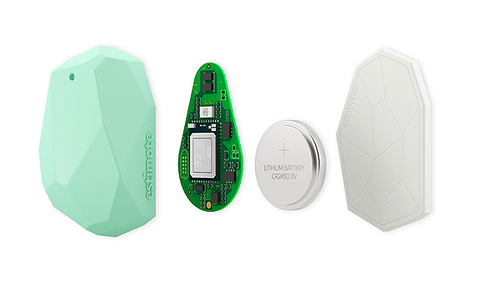
\includegraphics[width=0.6\textwidth]{img/estimote_beacon}
		\par\end{centering}
	\caption{Parts of Estimote beacon (source: \cite{RMPFEB})\label{fig:PartsOfEstimoteBeacon}}
	\label{fig10}
\end{figure}

Another important thing to note, Beacons are not connected to the Internet and do not collect any data from devices around them. Meaning all the data have to be processed in another device, most commonly a smartphone, and it also makes Beacon safe to use because there is no need to worry about sensitive data theft \cite{10TABB}.

\subsubsection{WiFi access-points}\label{subsec:WiFi access-points}
WiFi signals are commonly used in indoor localization due to their presence almost anywhere. In this case several WiFi transmitters of the \verb|eduroam| network made by Cisco were used. They are permanently deployed on every floor of a test building and cannot be influenced or changed.

\section{Server}\label{sec:Server}
Implemented application do not necessarily need a server for its core functionality but it is common and faster to run an analysis of the data and other heavy computational work on a different, faster device. Functionality of the server is to serve as a backup of the data and also as a synchronization point to enable other devices to download fingerprints and upload new ones.

The server infrastructure was built in previous years \cite{IILUBLEB} but it was improved for this solution. It uses NoSQL database to save fingerprints. This type of database does not have fixed scheme, making it easy to save all kinds of data. There are many NoSQL databases, around 250 at this time, to choose from. Selected database is called Couchbase, it saves data in JSON files with its own query language similar to SQL. Part of this database can also replicate data between other devices which could be used in the application part. In the end it was deemed too slow and data heavy for usage in the application, creating the need for creation of a middleman API between Android application and Couchbase database.

As \fref{fig057} shows server has three main parts to work with. First, already mentioned is Couchbase database to keep scanned data. Second, sync gateway that can synchronize data between devices, not used in this implementation. Both of these part were already implemented in previous years \cite{IILUBLEB}. Final part is web application working as a REST API to send data between the server and mobile application. 

This API is written in Java based framework called Spring to keep the code similar to Android. It was documented using Swagger and it handles two main HTTP routes: \verb|fingerprints| and  \verb|fingerprints-meta|. Before any tasks are issued, mobile application checks data on the server using \verb|fingerprints-meta| route which returns count of new fingerprints and last time specific device saved fingerprints on the server. With this information the application knows how many fingerprints to upload and download, in this specific order, to ensure data is stored first. To prevent device memory exhaustion and connection timeout both of these tasks have specific limits, download can process 100 of fingerprints while upload only 20. Server can also generate data files for analysis, split by technology, time, origin device and other filters. To simplify this generation it is similar loading all fingerprints, meaning it does not create file but prints the data directly into the connection stream.

One last thing to note in \fref{fig057} is the connection with sync gateway. Even though it is not used in this implementation for synchronization it is used to save fingerprints into the database. When data is saved into Couchbase directly sync gateway will not display them, that is why the upload must go through the gateway. This is to ensure all previous and next solution can use this feature without loosing any important data.

\section{Application Software}\label{sec:ApplicationSoftware}
Software part for smartphone and smartwatch uses Android system which was already described in \hyperref[sec:Android]{Chapter 3}. This section will provide basic information about libraries, technologies and systems used in such applications.

\subsection{AltBeacon Library}\label{subsec:AltBeaconLibrary}
Since Android core does not allow scanning for BLE beacons this feature must be implemented in a library extending system features. There are multiple solutions that can be used to scan for beacons such as Estimote SDK \cite{ESDKfA} which was already used in previous thesis \cite{PMRIL}. To change things up BLE beacons are found via AltBeacon Library \cite{ABL}.

Since there was no open and inter-operable specification for proximity beacons, Radius Networks has created the AltBeacon specification as a proposal to solve this issue. It is an open and free specification for BLE beacons with focus to create an open, competitive market for implementation of these devices \cite{AltB}. Basic configuration of this library can scan for beacons based on this standard and it also supports Eddystone beacons which is Google's open source format. To support already mentioned Estimote beacons this library configuration must be altered to support their detection. Luckily this function can be easily modified to support different kinds of beacons by just one following line of code \cite{ABL, EDDF}.

\begin{lstlisting}[caption=Code to enable all beacon types]
beaconManager.getBeaconParsers().add(
	new BeaconParser().setBeaconLayout("m:2-3=0215,i:4-19,
		i:20-21,i:22-23,p:24-24"));
\end{lstlisting}

This library uses publish-subscribe design pattern, meaning one scan data is send to multiple clients if they listen for them. Using this approach has an advantage of eliminating the need to run a scan per client. Update to Android 8 introduced a bug in this feature making it unable to confirm the registration of client so the scanner has to be reworked thus postponing the data collection and analysis.

\subsection{Database}\label{subsec:Database}
This solution makes use of two different types of databases to store all the Fingerprint data for calculations. First, is SQLite database implemented in Android mobile application to save Fingerprints from smartphone and smartwatch. This database is default implementation and most commonly used in Android applications. Second database type is Couchbase implemented on the server \verb|beacons.uhk.cz| to keep all Fingerprint data in one place and this enable synchronization and data analysis.

\subsubsection{SQLite database}\label{subsec:SQLiteDatabase}
SQL (Structured Query Language) is a standard language for storing, manipulating and retrieving data in databases. It is a type of Relational Database, meaning all data is saved into tables with specified rows and columns \cite{WISQLITE}. These tables usually have set amount of rows with specific names that protect from adding wrong data, for example you cannot add data \verb|Person(name, surname, eye color)| into table \verb|Person(name, surname)| because there is no column named \verb|eye color| in the table.

Structured data is one of the advantages of this database type and it makes calculation faster but usually uses more storage space. Other advantage is that data can be only saved once since they can be connected to each other. It supports complex queries for creating, reading, updating and removing data (CRUD) and better security with user and table management. Some disadvantages of this system can be with complexity and inflexibility of database scheme because it is hard to setup and does not allow other data then is defined in the tables \cite{ERDMS}. Altering schemes in the future can be really complex since there is the need to parse all previous data to the new tables which does not need to have the same scheme as previous ones.

Since SQL with all the features can consume a lot of hardware resources for a smartphone that is not as fast as a server Android decided to implement SQLite. SQLite has the following noticeable features: self-contained, serverless, zero-configuration, transactional \cite{WISQLITE}.

\begin{itemize}
	\item Serverless = does not need second process for the server.
	\item Self-Contained = requires minimal support from operating system.
	\item Zero-configuration = no need for installation or any configuration.
	\item Transactional = data are protected against failed changes (application crashes, power failure, ...).
\end{itemize}

\subsubsection{Couchbase database}\label{subsec:CouchbaseDatabase}
Since SQL based databases can be complex to implement, scale and consuming more data storage space there was a drive to create so called NoSQL databases. Their most important feature is not having a scheme, that makes them easy to scale, and easy to replicate between multiple devices. There are around 225 NoSQL databases at this time and Couchbase is one of them \cite{NOSQLDB}.

Couchbase is distributed, document-based database with its own querying language called N1QL. It is a database focused on simple server configuration and easy use for clients and with built in caching layer and distribution system it does not require any changes in the application. There can be either one server instance of Couchbase or multiple of them can be connected and create a database cluster that holds all the data in multiple location (nodes) \cite{GSWCBS}.

Since SQL is used for decades and it became standard for working with data in databases this approach was extended for usage with JSON and called N1QL. It has all features of the SQL with only difference of being focused on JSON files that has no structure and it is used in Couchebase \cite{WINQL}.

There is a version of Couchbase for mobile called Lite that provides APIs to work with the documents and synchronize with the server instance. Problem of this solution is that Lite version does not implement N1QL and maps data as document views that have to instanced and usually use more data, at least on Android. 

\subsubsection{Comparison}\label{subsec:Comparison}
Both of these database solutions were tested on Android and SQL proved as a better solution. Not only it takes less storage space it is also able to load data faster. As \tref{tab3} shows SQL lite takes less data space and is almost three times faster in loading all the documents.

\begin{table}[h]
	\begin{center}
		\begin{tabular}{| l | c | c |}
			\hline
			Database type & Data size & Loading speed (315 documents) \\ \hline
			SQLite & 15MB & 23 second \\ \hline
			Couchbase without views & 31MB & 65 seconds \\ \hline
			Couchbase with views & 91MB & 65 seconds \\ \hline
		\end{tabular}
		\caption{Couchbase vs SQLite (sources: \cite{LGWSP, LGWST, HW2, PM600, AZW3})}
		\label{tab3}
	\end{center}
\end{table}

As shown SQL comes up better but it does not support any data synchronization so there must be custom solution created. If Couchbase Lite would have faster query time it would be preferable solution but it is not at this time.

\subsection{TileView}\label{subsec:TileView}
There are multiple ways to display map image in Android but the main ones have problems while displaying a big image because they will run out of memory. So it is usually better to try custom library or widget created specifically for displaying big image. There is multiple 2D and 3D libraries to display such an image but most of them display image as a whole meaning one big image file. 

There is another way introduced by Google Maps where map is displayed using small images so called \verb|tiles|. Image is cut into small pieces which is better for device memory management than one big image. Depending on how big the cuts are it can also display multiple zoom levels keeping the map quality high with high and low levels.

% Example of this and how to do it

\section{Application structure}\label{sec:ApplicationStructure}
This section describes structure of the applications and since there are two parts of this application (mobile and wear) both of them will be described.

\subsection{Mobile application}\label{subsec:MobileApplication}
Mobile application is the bigger and more complex part that handles scanning, map display and synchronization with the server.

\subsubsection{Activities}\label{subsec:Activities}
Activities are visible screens of the application. They serve as the entry point for a user's interaction with an application, and are also central to how a user navigates within an application (as with the Back button) or between apps (as with the Recents button) \cite{AD}.

Main activity for this application is called \verb|ScanActivity|. It displays map with proper building, floor and found Fingerprint in that specific location. It enables users to scan for new beacons and thus create new Fingerprints. Map and controls are implemented using TileView widget that was described in previous section. 

\subsubsection{Model}\label{subsec:Model}
Model package contains most important classes of the application and it's split into four parts called: adapters, configuration, database and tasks.

\paragraph{Adapters}\label{subsec:Adapters}\mbox{} \\
Adapters information. 

\paragraph{Configuration}\label{subsec:Configuration}\mbox{} \\
Configuration classes contain settings of the application. It uses Android's shared preferences that are key-value (xml) files to save small amount of application data. Each SharedPreferences file is managed by the framework and can be private or shared. One thing to note is that these files are not encrypted so it is not good to save user sensitive data in them.

\paragraph{Database}\label{subsec:Database}\mbox{} \\
Database package contains all classes needed for communication between application and SQL database. First part of this package are Fingerprints classes that correspond with tables and columns of the database. Second part are so called database helpers that handle communication between the application and SQLite database such as tables creation, selects, inserts, updates and deletions.

\paragraph{Tasks}\label{subsec:Tasks}\mbox{} \\
Tasks contain the most complex classes of this application and that is the Fingerprint scanner that has multiple sub-classes to parse all the necessary data from the scan. Tasks also contain connection with the server for data synchronization and Fingerprint transfers.

\subsubsection{Utilities}\label{subsec:Utilities}
Utilities contain classes not fit to any other category or classified as support ones which usually means classes for animations or warning messages but since this application communicates with the wear device this package also contains classes that handle such communication.

\subsection{Wear application}\label{subsec:WearApplication}
Wear application is simplified version of its smartphone counterpart. It handles only scanning, display of scanning progress and sending the data to the phone. 